\PassOptionsToPackage{table}{xcolor}
\documentclass[a4paper, twoside, openright, 12pt]{bhamthesis}

% \usepackage[top=2.5cm,bottom=2cm, right=2.5cm, left=2.5cm]
% {geometry} % Required to change the page size to A4

%% Spacing 
%
\usepackage{setspace}
\usepackage{enumitem}
\usepackage{xspace}
\setlist{nosep}

%% Fonts
%
\usepackage[T1]{fontenc}

%% Colours 
%
\usepackage[usenames,dvipsnames,svgnames]{xcolor}

%% Graphics
%
\usepackage{graphicx}
\graphicspath{{imgs/}}


%% Figures
%
\usepackage[caption=false]{subfig}
\renewcommand{\figurename}{Figure}


%% Titles
%
% if you want to change the look of the chapter/section/etc titles, use
% \usepackage{titlesec}


%% Tikz
%
% for drawings
\usepackage{tikz}


%% Tables
%
\usepackage{array, multirow}
\usepackage{colortbl}
\usepackage{booktabs}

%% Maths
%
\usepackage[cmex10]{amsmath}
\usepackage[standard]{ntheorem}
\usepackage{amsfonts}
\usepackage{textcomp}

%% Headers
%
\usepackage{fancyhdr}
\fancyhead[LO]{\nouppercase\leftmark}
\fancyhead[LE]{\nouppercase\rightmark}
\chead{}
\fancyhead[R]{\thepage}
\lfoot{}
\cfoot{}
\rfoot{}

%% Code
%
\usepackage{algorithm}
\usepackage{algorithmic}
% if using tcolorbox, load minted with it
% otherwise load it straightforward
% if using minted, add -shell-escape to 
% compile arguments
%\usepackage{minted}
%\usepackage[minted]{tcolorbox}


%%  HYPHENATION
%
\usepackage{hyphenat}
% explicitly hyphenate words here
%\hyphenation{transceiv-er im-ple-ment-ed mi-cro-con-trollers de-fined pa-ram-e-ter}


%%%% Titlepage %%%%
%%
\title{Thesis title}
\author{Jane Doe}
\date{\today}
\degree{\scshape Master of Science}
\school{School of Computer Science} 
\university{University of Birmingham}

%% PDF, URL and hyperlink
%
\usepackage{url}
\usepackage{afterpage}
\usepackage[pdftex,
            bookmarks=true,
            plainpages=false,
            naturalnames=false,
            colorlinks=true,%,
            pdfpagelabels,
            pdfstartview=FitH,breaklinks,
            linkcolor=black,citecolor=blue,urlcolor=blue]
        {hyperref}

%% Lorem ipsum
\usepackage{lipsum}

\begin{document}

\pagenumbering{Alph}
\frontmatter
\begin{titlepage}
\thispagestyle{empty}
\maketitle
\end{titlepage}

\newpage
\textcolor{white}{blank}
\newpage

\chapter*{Acknowledgements}
\thispagestyle{empty}
I would like to thank my cat.

\chapter*{Abstract}
\thispagestyle{empty}
\lipsum[1-3] 

\newpage

\pagestyle{empty}
\clearpage

\tableofcontents

\mainmatter

\hypersetup{pageanchor=true}
\pagenumbering{arabic}
\setcounter{page}{1}

\chapter{One}%
\label{chap:one}
\thispagestyle{empty}

We've used lipsum to fill in the space \cite{lipsum}.

\lipsum[4]

\section{This is a section}%
\label{sec:one:section_one}

\lipsum[5]

\begin{figure}
	\centering
  \resizebox{0.6\linewidth}{!}{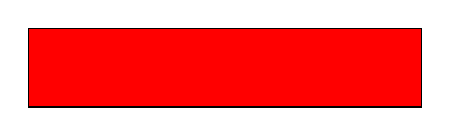
\begin{tikzpicture}
\draw[fill=red] (0,0) rectangle (5,1); 
\end{tikzpicture}
}
	\caption{This is an image.}
	\label{fig:image1}
\end{figure}

\lipsum[6-7]


\section{This is another section}%
\label{sec:one:section_two}

\lipsum[8-10]

\chapter{Two}%
\label{chap:two}
\thispagestyle{empty}

\lipsum[11]

\section{This is the first section of the second chapter}%
\label{sec:two:section_one}

\lipsum[12-13]

\subsection{And this is a subsection}%
\label{subsec:two:section_one:subsec_one}

\lipsum[14-15]

\subsection{Yet another subsection}%
\label{subsec:two:section_one:subsec_two}

\lipsum[16-18]

\section{This is the second section of the second chapter}%
\label{sec:two:section_two}

\lipsum[19-20]


\bibliographystyle{bhamthesis}
\bibliography{bib_file}
\end{document}
